\documentclass[fleqn,leqno,11pt,letterpaper,final]{article}
%----README----
% This TeX file was automatically generated by GNU Emacs's Org Mode.
% For better documentation refer to the corresponding Org file, 
% which you can find in the sources specified bellow.
% Do keep in mind that this file undergoes little to none manual revision.
%----LICENSE---
% Copyright 2021 Jhonny Lanzuisi (jalb97@gmail.com)
% More source files at github.com/JLanzuisi
%
% This program is free software: you can redistribute it and/or modify
% it under the terms of the GNU General Public License as published by
% the Free Software Foundation, either version 3 of the License, or
% (at your option) any later version.
%
% This program is distributed in the hope that it will be useful,
% but WITHOUT ANY WARRANTY; without even the implied warranty of
% MERCHANTABILITY or FITNESS FOR A PARTICULAR PURPOSE.  See the
% GNU General Public License for more details.
%
% You should have received a copy of the GNU General Public License
% along with this program.  If not, see <https://www.gnu.org/licenses/>.
%--------------

\hfuzz1pc
\overfullrule=2cm

\usepackage[spanish,es-noindentfirst]{babel}
\usepackage{csquotes}

\usepackage
[
	includehead,
	includefoot,
	top=.5cm,
	bottom=.5cm,
	left=1.7cm,
	right=7.3cm,
	marginparsep=0.5cm,
	marginparwidth=7cm,
]
{geometry}

\usepackage{mathtools}
\DeclareMathOperator{\Rea}{Re}
\DeclareMathOperator{\Ima}{Im}
\DeclareMathOperator{\car}{car}
\DeclareMathOperator{\traz}{tr}
\DeclareMathOperator{\gen}{gen}
\DeclareMathOperator{\mcm}{mcm}

\usepackage{unicode-math}

\setmainfont{New Computer Modern Book}
\defaultfontfeatures{Scale=MatchLowercase}
\setsansfont{Public Sans}
\setmonofont{Average Mono}
\newcommand{\headfont}{\sffamily}

\frenchspacing
\linespread{1.05}

\setmathfont{New Computer Modern Math}

\usepackage[final]{microtype}

\PassOptionsToPackage{final}{graphicx}
\PassOptionsToPackage{dvipsnames}{xcolor}

\usepackage
{
	xcolor,
	graphicx,
	cancel,
	booktabs,
	hyphenat,
	authoraftertitle,
	pdfpages,
	metalogo
}

\usepackage
[
backend=biber,
backref=true,
citestyle=authoryear-comp,
style=chicago-authordate ,
sorting=ynt
]
{biblatex}
\addbibresource{/home/jhonny/git/Misc-LaTeX-files/bib/general.bib}

\usepackage{url} 
\usepackage{hyperref} 
\definecolor{Carmine}{HTML}{960018}
\newcommand{\linkcolor}{Carmine}
\hypersetup
{
colorlinks=true,
linkcolor=\linkcolor,
urlcolor=\linkcolor,
citecolor=\linkcolor
}
\usepackage[spanish,nameinlink]{cleveref}

\newcommand{\marfont}{}

%\renewcommand*{\marginfont}{\marfont}
\let\oldmarginpar\marginpar
\renewcommand
	{\marginpar}
	[1]
	{
	\oldmarginpar{\raggedright\marfont #1}
	}

\newcounter{nota}
\newcommand
	{\nota}
	[1]
	{
	\refstepcounter{nota}\textsuperscript{\thenota}
	\marginpar{
		\raggedright\itshape\thenota. #1
		}
	}

\renewcommand{\footnote}{\nota}

\usepackage{enumitem} 
\setlist[enumerate]{left=-11pt,nosep}
\setlist[description]{font=\normalfont,leftmargin=\parindent}
\setlist[itemize]{label={\small\textbullet},left=-11pt}

\newcommand{\Asignatura}{}
\newcommand
	{\asignatura}
	[1]
	{\renewcommand{\Asignatura}{#1}}

\makeatletter
\def\@maketitle
	{
	\newpage
	\null
	\let \footnote \thanks
  	\begin{flushleft}\sffamily
  	\marginpar
		{
		\vspace*{.2em}
		\begin{minipage}{.7\marginparwidth}
		\begin{center}
		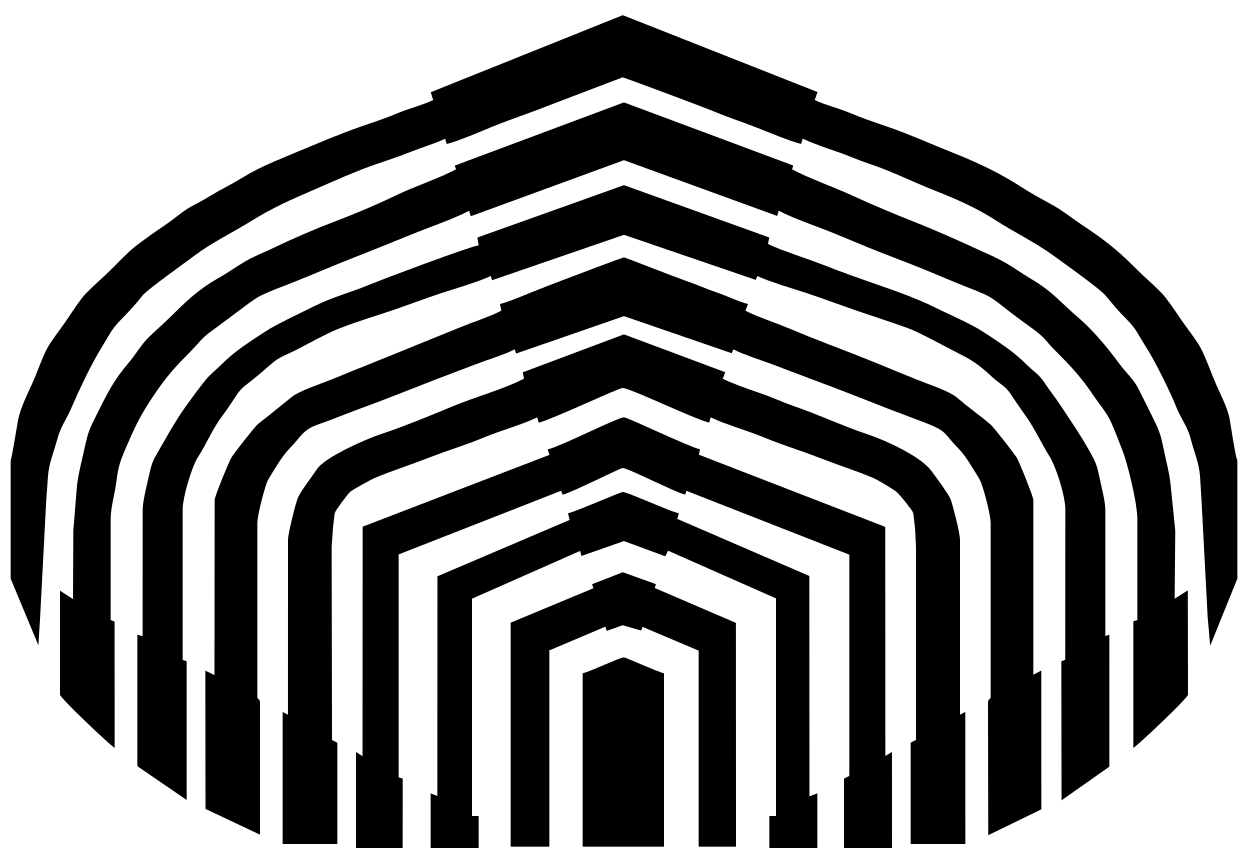
\includegraphics
			[width=.35\marginparwidth]
			{/home/jhonny/git/LaTeX-University/usb-logo.png}\\
		Universidad Simón Bolívar\\
		Caracas, Venezuela\\
		\end{center}
		\end{minipage}
		}
	{
	\Large\headfont
		\MyTitle
	\par
	}
	\smallskip
	\Asignatura\par
	\smallskip
	\@author,\ \today.
	\end{flushleft}
	\vskip 1.5\baselineskip
	}
\makeatother

\usepackage[final]{listings} 
\lstset
{
numbers=left, numberstyle=\tiny\ttfamily, stepnumber=2, numbersep=5pt, 
basicstyle=\ttfamily, 
stringstyle=\ttfamily,
commentstyle=\itshape,
breaklines=true,
postbreak=\mbox{$\hookrightarrow$\enspace},
columns=flexible
}

\usepackage{caption} 
\captionsetup
{
font={rm},
justification=raggedright,
singlelinecheck=false,
skip=3pt
}

\usepackage[explicit]{titlesec}

\titleformat{\section}[hang]
	{\flushleft\headfont}
	{\addfontfeatures{Numbers=Lining}\thesection}
	{1em}
	{\addfontfeatures{LetterSpace=5}\MakeUppercase{#1}}
	[]
\titlespacing*{\section}
	{0em}
	{1.5\baselineskip}
	{.5\baselineskip}
\titleformat{\subsection}
	{\flushleft\sffamily}
	{\addfontfeatures{Numbers=Lining}\thesubsection}
	{.5em}
	{#1}
	[]
\titlespacing*{\subsection}
	{0em}
	{1\baselineskip}
	{1\baselineskip}
\titleformat{\paragraph}[runin]
	{\scshape}
	{}
	{0em}
	{\MakeLowercase{#1}}
	[.]
\titlespacing*{\paragraph}
	{0em}
	{1\baselineskip}
	{5pt}

\let\oldtoc\tableofcontents
\renewcommand
{\tableofcontents}
{\marginpar{\bigskip\oldtoc}}
\usepackage{titletoc}

\titlecontents{section}
	[0em]
	{\vspace{0pt}}
	{\contentsmargin{0pt}}
	{\contentsmargin{0pt}}
	{\contentspage}
	[\vspace{.3em}]
\titlecontents{subsection}
	[1.5em]                              
	{\vspace{0pt}}
	{\contentsmargin{0pt}\small}
	{\contentsmargin{0pt}\small}        
	{\small\contentspage}                 
	[\vspace{.3em}]

\usepackage{fancyhdr}

\renewcommand{\headrulewidth}{0pt}
\setlength{\headheight}{14pt}

\pagestyle{fancy}
\fancyhf{}
\fancyhead
	[L]
	{
	\ifodd\value{page}\MyTitle\else\Asignatura\fi
	}
\fancyhead[R]{\thepage}
\fancypagestyle
	{plain}
	{
	\fancyhead[R]{}
	\fancyhead[L]{}
	\fancyfoot[R]{}%
	\fancyfoot[L]{}
	\fancyfoot[C]{}
	}

\usepackage[thmmarks]{ntheorem}
  % \usepackage[thmmarks]{ntheorem}
  % 	\theoremstyle{plain}
  % 	\theoremindent0cm
  % 	\theorempreskip{0cm}
  % 	\theorempostskip{0cm}
  % 	\theoremheaderfont{\hspace*{\parindent}\upshape}
  % 	\theorembodyfont{\itshape}
  % 	\theoremseparator{.}
  % 	\newtheorem{teo}{Teorema}[section]
  % 	\newtheorem{cor}{Corolario}[teo]
  % 	\newtheorem{prop}{Proposición}[section]
  % 	\newtheorem{lem}{Lema}[section]
  % 	\theoremstyle{nonumberplain}
  % 	\theoremheaderfont{\normalfont}
  % 	\theorembodyfont{\upshape}
  % 	\newtheorem{proof}{Demostración}
  % 	\theoremstyle{plain}
  % 	\theorempreskip{1em}
  % 	\theorempostskip{1em}
  % 	\theoremheaderfont{\upshape}
  % 	\theorempostwork{\noindent}
  % 	\newtheorem{definition}{Definición}[section]

\theoremstyle{plain}
\theorempreskip{\medskipamount}
\theorempostskip{\medskipamount}
\theorembodyfont{\upshape}
\theoremseparator{.}
{
\theoremheaderfont{\itshape}
\newtheorem{definition}{Definición}
}
{
\theoremheaderfont{\scshape}
\newtheorem{theorem}{Teorema}
}


\title{Segundo Parcial}
\author{Jhonny Lanzuisi, 15\,10759}
\asignatura{Análisis 1}
\begin{document}
\maketitle
\tableofcontents
% Este es el primer parcial de algo.
\section{Primer ejercicio}
Demostrar que una sucesión real $\{ a_n \}_{n\in\mathbb{N}}$ es convergente a$a$ un valor $L$ real si, y
sólo si, toda sub-sucesión de\textsf{a} a $\{ a_n \}$ es convergente al valor $L$.

\subsection{Solución}

Sea $\{ a_{n_k} \}$ una subsucesión de $\{ a_n \}$ 
supongamos que $\{ a_n \}$ converge a $L$. Entonces, dado $\epsilon>0$, existe un $N\in\mathbb{N}$ tal que
\begin{align}\label{eq1}
	\left\lvert  a_n - L \right\rvert<\epsilon
\end{align}
para todo $n>N$.

Como $\{ a_{n_k} \}$ es una subsucesión de $\{ a_n \}$ se tiene que los índices $n_{k}$ son
un subcojunto de los índices $n$. Por lo tanto, para todo $n_{k}>N$, debe cumplirse que
\[
	\left\lvert a_{n_k}-L \right\rvert<\epsilon
\]
pues de lo contrario estos índices $n_k$ serían ciertos naturales $n>N$ para los cuales
no se cumpliría~\ref{eq1}. Se tiene entonces que $\{ a_{n_k} \}$ converge a $L$ como se
buscaba.

\marginnote{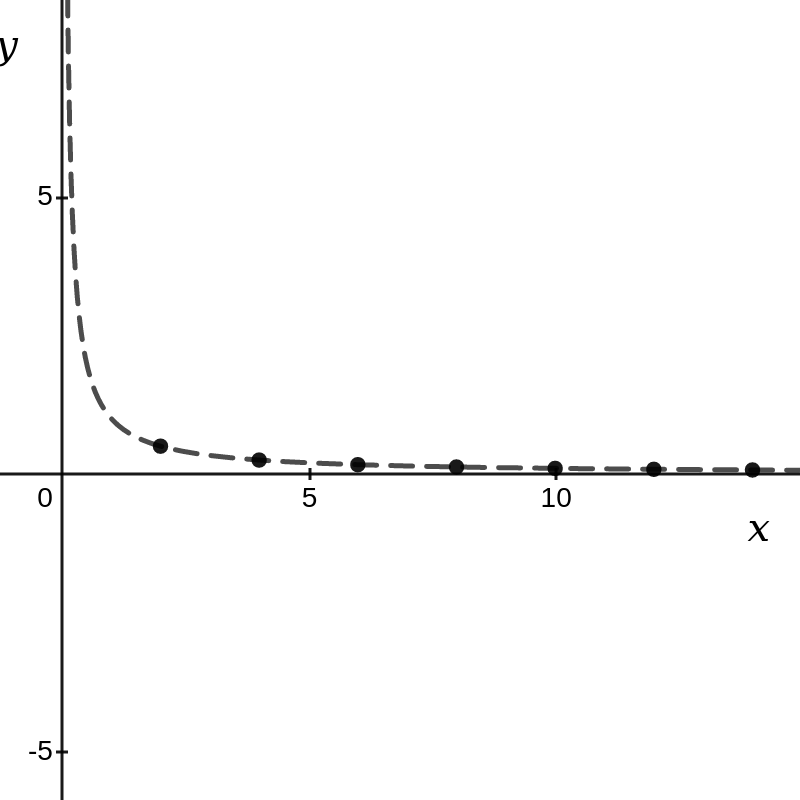
\includegraphics[scale=.2]{p1.png}\\ Ejemplo de una sucesión convergente
		($a_n=1/n$) y una subsucesión (solo los n pares) convergente al mismo
		límite (0).
}
Supongamos ahora que toda subsucesión $\{ a_{n_k} \}$ de $\{ a_n \}$ converge a $L$.
Entonces el resultado se sigue de forma casi inmediata puesto que $\{ a_n \}$ es una
subsucesión de ella misma. Mas explícitamente, $\{ a_n \}$ es la subsucesión que se obtiene
al tomar todos los índices $n$ en el mismo orden que aparecían originalmente, entonces
nuestra hipótesis nos da que $a_n$ converge.

\section{Segundo ejercicio}%
\label{sec:Segundo ejercicio}
Demostrar que $a\in A'$ si, y sólo si, existe una sucesión $\{ x_n \}_{n\in\mathbb{N}}$ en $A$ tal que
$ \lim_{n \to \infty} \{ x_n \}=a$.

\subsection{Solución}
Supongamos que existe una sucesión $\{ x_n \}$ en $A$ que converge a $a$.
Entonces, dado $\epsilon>0$, existe un $N_\epsilon\in\mathbb{N}$ tal que
\[
	\left\lvert x_{n}-a \right\rvert<\epsilon
\]
para $n>N_\epsilon$.

Es decir, para todo $n>N_\epsilon$ todos los puntos de la sucesión $\{ x_n \}$ están contenidos
en la bola de radio $\epsilon$ y centrada en $a$. Como la convergencia de $\{ x_n \}$ asegura que lo
anterior se cumple para cualquier $\epsilon$ dado, se tiene que todo entorno del punto $a$ (toda
bola de radio $\epsilon$) contiene infinitos puntos de $A$ (los puntos de la sucesión) y,
por lo tanto, $a$ es un punto de acumulación de $A$\footnote{En el Apostol\cite{apostol_mathematical_1974}, pag. 53 Teorema 3.17}.

Supongamos ahora que $a$ es un punto de acumulación. Queremos ver que existe una
sucesión $\{ x_n \}$ que converge a $a$, esto lo haremos construyendo dicha sucesión

% \tikzset{every picture/.style={line width=0.75pt}} %set default line width to 0.75pt        
%\marginnote{ Entornos descendentes de $a$.\\
%	\begin{tikzpicture}[x=0.75pt,y=0.75pt,yscale=-1,xscale=1]
%	%uncomment if require: \path (0,300); %set diagram left start at 0, and has height of 300
	
%	%Straight Lines [id:da33306306965494015] 
%	\draw    (100,122) -- (267.67,122) ;
%	%Straight Lines [id:da32365339533662774] 
%	\draw    (259.67,112.67) -- (259.67,131.33) ;
%	%Straight Lines [id:da38315840975758275] 
%	\draw    (109.67,112) -- (109.67,130.67) ;
%	%Straight Lines [id:da1866954731177436] 
%	\draw    (185.67,112) -- (185.67,130.67) ;
%	%Straight Lines [id:da22553118858535703] 
%	\draw    (140.67,116.67) -- (140.67,129.33) ;
%	%Straight Lines [id:da8542397100763582] 
%	\draw    (230,116) -- (230,128.67) ;
%	%Straight Lines [id:da9330130533226818] 
%	\draw    (210.67,115.33) -- (210.67,128) ;
%	%Straight Lines [id:da7653796759032424] 
%	\draw    (160,116.67) -- (160,129.33) ;
	
%	% Text Node
%	\draw (98,135.33) node  [font=\small]  {$-r_{1}$};
%	% Text Node
%	\draw (270.67,138.67) node  [font=\small]  {$r_{1}$};
%	% Text Node
%	\draw (186.67,136.67) node  [font=\small]  {$a$};
%	% Text Node
%	\draw (232.33,135.33) node  [font=\scriptsize]  {$r_{2}$};
%	% Text Node
%	\draw (139.33,135.33) node  [font=\scriptsize]  {$-r_{2}$};
%	% Text Node
%	\draw (212.33,134.67) node  [font=\scriptsize]  {$r_{3}$};
%	% Text Node
%	\draw (160.33,136.33) node  [font=\scriptsize]  {$-r_{3}$};
%	\end{tikzpicture}
%}
Tomemos números reales positivos $r_1,r_2,\dots$ tales que
$r_1>r_2>\dots$
Y consideremos las bolas $B_{r_i}(a)$ con $i=1,2,\dots$
De esta manera se obtienen entornos de $a$ que son cada vez más pequeños.

%\marginnote{
%	\begin{tikzpicture}[x=0.75pt,y=0.75pt,yscale=-1,xscale=1]
%	%uncomment if require: \path (0,300); %set diagram left start at 0, and has height of 300
	
%	%Straight Lines [id:da33306306965494015] 
%	\draw    (100,122) -- (267.67,122) ;
%	%Straight Lines [id:da32365339533662774] 
%	\draw    (259.67,112.67) -- (259.67,131.33) ;
%	%Straight Lines [id:da38315840975758275] 
%	\draw    (109.67,112) -- (109.67,130.67) ;
%	%Straight Lines [id:da1866954731177436] 
%	\draw    (185.67,112) -- (185.67,130.67) ;
%	%Straight Lines [id:da22553118858535703] 
%	\draw    (140.67,116.67) -- (140.67,129.33) ;
%	%Straight Lines [id:da8542397100763582] 
%	\draw    (230,116) -- (230,128.67) ;
%	%Straight Lines [id:da9330130533226818] 
%	\draw    (210.67,115.33) -- (210.67,128) ;
%	%Straight Lines [id:da7653796759032424] 
%	\draw    (160,116.67) -- (160,129.33) ;
%	%Straight Lines [id:da22227714468718218] 
%	\draw    (247.11,117.33) -- (247,126.67) ;
%	%Straight Lines [id:da2882754094691373] 
%	\draw    (150.78,117) -- (150.67,126.33) ;
%	%Straight Lines [id:da8739024195762054] 
%	\draw    (198.44,117) -- (198.33,126.33) ;
	
%	% Text Node
%	\draw (98,135.33) node  [font=\small]  {$-r_{1}$};
%	% Text Node
%	\draw (274,138) node  [font=\small]  {$r_{1}$};
%	% Text Node
%	\draw (186.67,136.67) node  [font=\small]  {$a$};
%	% Text Node
%	\draw (247.67,132) node  [font=\scriptsize]  {$x_{1}$};
%	% Text Node
%	\draw (151.67,132) node  [font=\scriptsize]  {$x_{2}$};
%	% Text Node
%	\draw (199.67,133.33) node  [font=\scriptsize]  {$x_{3}$};
%	\end{tikzpicture}\\
%	Construcción de la sucesión $x_n$ convergente a $a$.
%}
Puesto que $a$ es un punto de acumulación todas las bolas $B_{r_i}(a)$ contienen al menos
un punto de $A$ distinto de $a$, llamemos a este punto $x_ix_j$. De esta manera se obtiene una
sucesión $x_n=x_1,x_2,\dots$ en $A$. Queda por ver que esta sucesión converge a $a$.

Sea $\epsilon>0$ un número real dado. Entonces podemos considerar dos casos:

\begin{description}
	\item[$\epsilon\geq r_1$] 
		En este caso la bola $B_\epsilon(a)$ contiene a $B_{r_1}(a)$. 
		Y, por la construcción anterior, todos los puntos de la sucesión $\{ x_n \}$
		pertenecen a la bola de radio $\epsilon$. Es decir, para todo $n>1$
		\[
			\left\lvert x_n-a \right\rvert<\epsilon
		\]
		y se tiene que $\{ x_n \}$ converge a $a$.
	\item[$\epsilon\leq r_1$] 
		En este caso la bola $B_{\epsilon}(a)$ esta contenida en la bola de radio
		$r_1$. Como los $r$ se elegieron de manera descendente, tomemos el primer
		$r_k$ tal que $\epsilon>r_k$ 
		(Este $r_k$ existe pues, de lo contrario, $\epsilon\neq 0$ sería un mínimo del intervalo $(0,r_1)$ lo cual es imposible).
		Entonces $B_{r_k}(a)\subset B_\epsilon(a)$ y, por la forma en la que se contruyó la
		sucesión $\{ x_n \}$, todos los puntos de la sucesión tales que $n>k$ están
		en la bola de radio $\epsilon$. Dicho de otra forma, para todo $n>k$
		\[
			\left\lvert x_n-a \right\rvert<\epsilon,
		\]
		y $\{ x_n \}$ converge a $a$.
\end{description}

\section{Cuarto Ejercicio}%
\label{sec:Cuarto Ejercicio}
Sea $ \sum_{n=1}^{\infty}a_n $ una series de términos positivos y sea
\[
	L= \lim_{n \to \infty} \frac{\log(1/a_n)}{\log(n)}.
\]

Demuestre que la serie converge si $L>1$ y que diverge si $L<1$.

\subsection{Solución}
Supongamos que $L<1$. Entonces, cuando $n\to\infty$ se tiene que,
\[
	\frac{\log(1/a_n)}{\log(n)} < 1
\]
esto implica, multiplicando por $\log(n)$,
\[
	\log\left( \frac{1}{a_n} \right) < \log(n)
\]
y como el logaritmo es una función continua y creciente, esto
a su vez implica que
\[
	\frac{1}{a_n} < n
\]
y, finalmente,
\[
	a_n> \frac{1}{n} 
\]
y la divergencia de la serie armónica implica la divergencia de $a_n$.

Supongamos ahora que $L>1$ pero que $L<\infty$, digamos que es igual a un valor $C$.
Entonces, cuando $n\to\infty$,
\[
	\frac{\log(1/a_n)}{\log(n)} = C,
\]
de donde se deduce, al igual que antes, que
\[
	a_n= \frac{1}{n^C} 
\]
puesto que $C\log(n)=\log(n^C)$.

Como $C>1$ la serie de $1/n^C$ converge y por lo tanto $a_n$ también converge.

\section{Quinto Ejercicio}%
\label{sec:Quinto Ejercicio}
Dada la serie
\[
	\sum_{n=1}^{\infty} \frac{1}{n^{\alpha}}\quad (\alpha>0)
\]
Determine los casos para los cuales la serie converge o diverge.

\subsection{Solución}
Consideremos la función $f(x)=1/x^{\alpha}$ donde $x,\alpha$ son reales tales que $\alpha>0$
y $x>1$. Como $x>1$ es claro que la función decrece a cero. Por lo tanto, podemos
utilizar el criterio de la integral para determinar la convergencia de la serie.

Veamos entonces la sucesión $t_n$ dada por
\[
	t_n=\int_1^n x^{-\alpha} dx=
	\begin{cases}
		\dfrac{n^{1-\alpha}-1}{1-\alpha} &\text{si}\;\alpha\neq1\\
		\log(n) &\text{si}\;\alpha=1.
	\end{cases}
\]

Si $\alpha>1$ entonces el término $n^{1-\alpha}$ tiende a cero cuando $n\to\infty$.
\marginnote{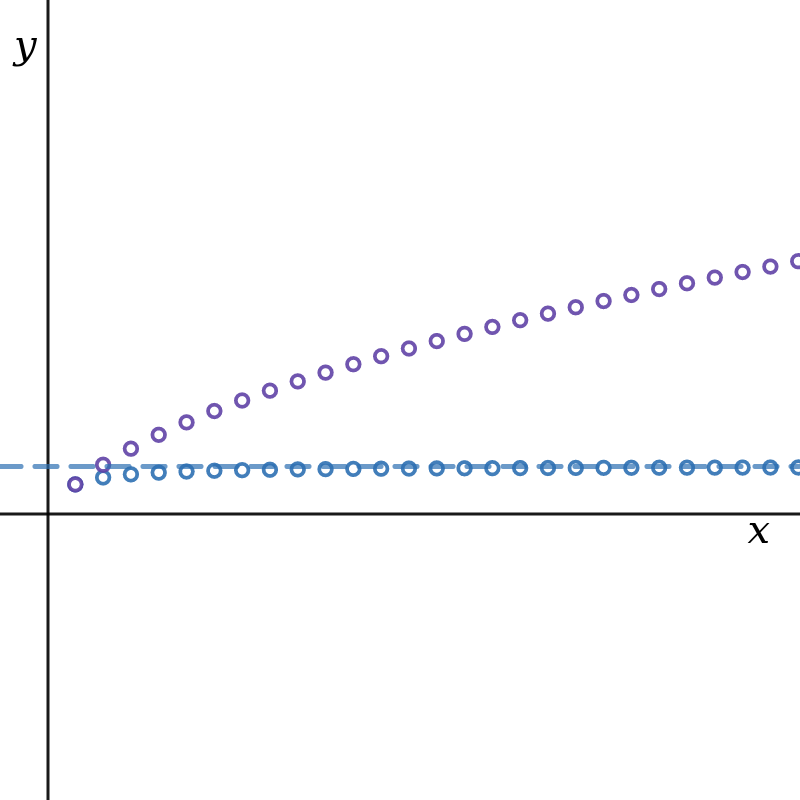
\includegraphics[scale=.2]{p3.png}\\ Ejemplo 
	de los valores $\alpha=1/2$ (morada) y $\alpha=2$
	(azul). La primera serie es divergente y la segunda
	converge a $\pi^2/6\footnotemark$ (línea azul).
}
\footnotetext{Este hecho lo demostro Euler en 1735}
Por lo cual la sucesión $t_n$ converge y el criterio integral nos
da como resultado que nuestra serie original también converge.

Si $\alpha<1$ entonces $n^{1-\alpha}$ tiende a infinito cuando $n\to\infty$.
Por lo que la sucesión $t_n$ diverge y el criterio integral
asegura que nuestra serie original también diverge.

Si $\alpha=1$ se obtiene la serie armónica que diverge.
Para ver la divergencia de la serie armónica notemos que
la sucesión $t_n=\log(n)$ diverge al no estar acotada.

\section{Sexto Ejercicio}%
Demostrar que si la serie $ \sum_{n=1}^{\infty} a_n$ es convergente, entonces
\[
	\sum_{n=1}^{\infty} \frac{\sqrt[]{a_n}}{n}  
\]
también converge.

\subsection{Solución}
Notemos que 
\[
	\frac{\sqrt[]{a_n}}{n} = \sqrt[]{ \frac{a_n}{n^2} }= \sqrt[]{a_n\left( \frac{1}{n^2}  \right)}
\]
Entonces, la desigualdad entre la media aritmética y la geométrica%
\footnote{Ver~\cite{spivak_calculus_2008}. Capítulo 1, ejercicio 7, p.28}
nos da que
\marginpar{Una prueba de ocmo se ve la fuente en los amrgenes hay que escribir tonteri a aqui un rato pa probar}
\[
	\sqrt{a_n\left( \frac{1}{n^2}  \right)} \leq \frac{a_n}{2}+ \frac{1}{2n^2}.
\]
donde la serie de $a_n/2$ converge dado que $a_n$ converge y la serie de $1/2n^2$ converge por el ejercicio anterior.

Se tiene entonces que la serie de $\sqrt[]{a_n}/n$ esta acotada por la suma de dos series convergentes, y por lo tanto converge.

\section{Séptimo ejercicio}%
\label{sec:Séptimo ejercicio}
Sea $\{ x_n \}$ una sucesión convergente a un valor $L$. Demuestre que
\[
	\lim_{n \to \infty} \frac{x_1+x_2+\dots+x_n}{n} 
\]
converge también a $L$. Determine si es cierto o no el recíproco.

\subsection{Solución}
Como $\{ x_n \}$ converge  a $L$ sabemos que, dado $\epsilon>0$, existe un $N\in\mathbb{N}$
tal que
\begin{align}\label{eq2}
	\left\lvert x_n-L \right\rvert<\epsilon
\end{align}

cuando $n>N$.

Llamemos $s_n$ a  
\[
	 \frac{x_1+x_2+\dots+x_n}{n} .
\]
Entonces queremos demostrar que existe algun $M\in\mathbb{N}$ para el cual se cumple que
\[
	\left\lvert s_n-L \right\rvert<\epsilon\quad (n>M).
\]

Notemos que, si tomamos un entero $m>N$,
\begin{align*}
	\left\lvert s_m-L \right\rvert 
		&= \left\lvert \frac{1}{m} \sum^{m}_{k=1} x_k - L\right\rvert\tag{$\ast$}
\end{align*}

Ahora, separamos la suma de la derecha en dos partes: una parte será una suma 
finita que \emph{no depende} de
$m$ y la otra una suma que si depende $m$ y que involucra a los enteros mayores que $N$, es
decir, justamente a esos enteros para los que se cumple~\ref{eq2}.
\begin{align*}
	(\ast) &= \left\lvert \frac{1}{m} \sum^{N-1}_{k=1} x_k-L + \sum^{m}_{N} x_k-L  \right\rvert\\	
	\shortintertext{y, por la desigualdad triangular,}
	       &\leq \left\lvert \frac{1}{m} \sum^{N-1}_{k=1} x_k-L \right\rvert + \left\lvert \frac{1}{m} \sum^{m}_{k=N} x_k-L \right\rvert\\
	       &= \frac{1}{m} \sum_{k=1}^{N-1} \left\lvert x_k-L \right\rvert + \frac{1}{m} \sum_{k=N}^{m} \left\lvert x_k-L \right\rvert
\end{align*}

Ahora, la suma de la izquierda es finita y por lo tanto esta acotada, digamos que por una
constante $C$. La suma de la derecha es una suma donde cada uno de los $m-N$ términos están
acotados por $\epsilon$ (debido a~\ref{eq2}). Se tiene entonces que lo anterior es
\marginnote{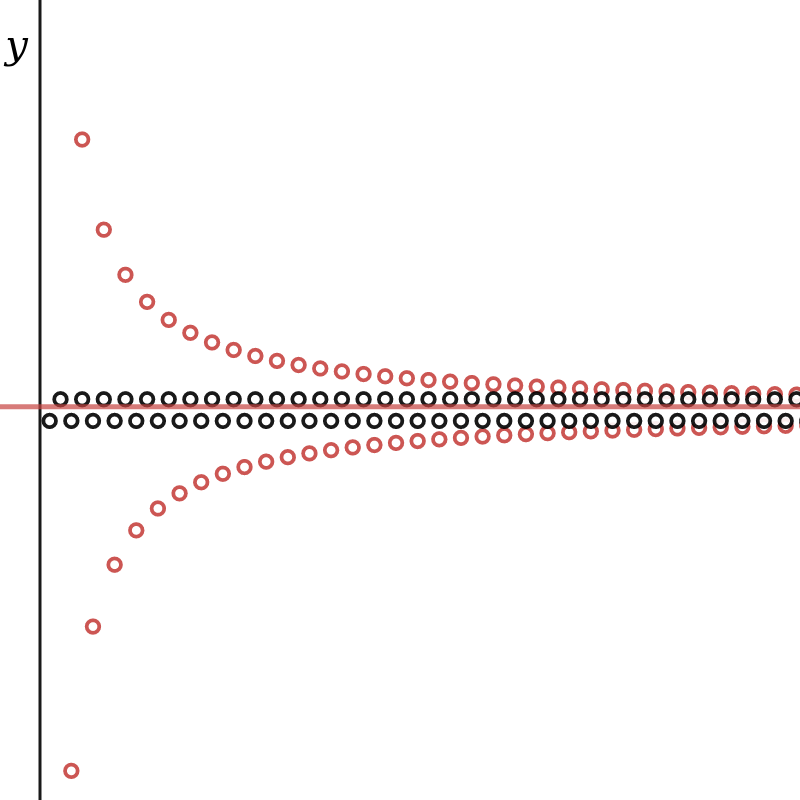
\includegraphics[scale=.2]{p2.png}\\ 
	La sucesión $(-1)^n$ (negro) y la serie de $(-1)^n/n$ (rojo)
	junto con la línea (rojo) $y=\log(2)$ a la cual converge la serie.
}
\[
	\phantom{(\ast)}\leq \frac{C}{m} + \frac{1}{m} (m-N)\epsilon
		= \frac{C}{m} + \epsilon- \frac{N}{m}\epsilon.
\]
Y, dejando $C,N$ fijos, podemos hacer que $m\to\infty$ para conseguir que
el lado derecho de la igualdad anterior tienda a $\epsilon$.

El recíproco \emph{no es cierto}. Para un contraejemplo, consideremos la sucesión
$\{ a_n \}=(-1)^n$. Esta sucesión no converge, sin embargo,
\[
	\lim_{n \to \infty} \sum_{k=1}^{n} \frac{(-1)^k}{k}  
\]
converge por criterio de Liebniz. Más aún, converge a $\log(2)$ por ser un caso
de la serie  logarítmica\footnote{Vease\cite{apostol_calculus._1980}. Sección 10.17}.


\printbibliography[
heading=bibintoc,
title={Referencias}
]
\end{document}
